\documentclass[a4paper,11pt]{article}

\usepackage[utf8]{inputenc}
\usepackage{booktabs, array, pdflscape}
\usepackage{geometry}
\usepackage{graphics,graphicx}
\usepackage{color}
\usepackage{url}
\usepackage{enumerate}

\usepackage[labelsep=period]{caption}
\usepackage{subcaption}

\setlength{\textheight}{24cm}  
\setlength{\textwidth}{15cm}
\setlength\oddsidemargin{0cm}
\setlength\evensidemargin{0cm}
\setlength\voffset{-1cm}

\renewcommand{\textfraction}{0.01}
\renewcommand{\floatpagefraction}{0.85}
\renewcommand{\topfraction}{0.8}
\renewcommand{\bottomfraction}{0.8}

\newcommand{\red}[1]{\textcolor{red}{#1}}	
\newcommand{\mc}[3]{\multicolumn{#1}{#2}{#3}}

\newcommand{\Ni}{({\em i\,})~}
\newcommand{\Nii}{({\em ii\,})~}
\newcommand{\Niii}{({\em iii\,})~}

\newcommand{\en}{$en$}
\newcommand{\es}{$es$}
\newcommand{\fr}{$fr$}
\newcommand{\de}{$de$}

%opening
\title{

\includegraphics[width=3cm]{./img/200px-SuitClubs.png} \\
\Huge M5.1 -- Intrinsic Evaluation of the \\ Machine Translation Engines \\ 
}
\author{\vspace*{1cm}\\ \LARGE Cristina Espa\~na-Bonet and \'Ad\'am Varga \medskip \\ \Large Universit\"at des Saarlandes}
\date{\vspace*{2cm} -- v1.2 --\\July 2018}


\begin{document}

\clearpage\maketitle
\thispagestyle{empty}

\vspace*{5cm}
\begin{abstract}
This document describes the statistical and neural machine translation systems used as baselines within the CLUBS project and their evaluation with automatic metrics. Those systems are trained with large out-of-domain and/or small in-domain corpora, which is described in deliverable M1.2.
\end{abstract}

\newpage
\tableofcontents
\clearpage

% guarrada, no va el \cleardoublepage
% \clearpage\mbox{}\clearpage

%\newpage
\section{Introduction}
\label{s:intro}

In the last years, statistical machine translation systems (SMT) have shown to offer a competitive translation quality when \emph{enough data} is available. When compared to rule-based translation systems (RBMT), SMT systems are cheaper and easier to build and they only rely on the existence of parallel corpus --preferably on the specific domain to translate-- in order to be trained. These advantages are common to all data-based systems. Recently, a new paradigm has been applied within data-based machine translation: neural machine translation (NMT). NMT systems have shown to outperform SMT systems for language pairs where huge amounts of parallel corpora are available~\cite{WMT1:2016,WMT2:2017}.

As always, there are pros and cons for using one family of systems or the other. SMT systems need less data to get a similar performance and can be trained in a desktop computer. On the other hand, the most modest NMT systems need at least one week of GPU time to get competitive results. A more detailed discussion is reported in deliverable M1.4.

In the CLuBS project we face two main issues. First, we want to translate among all four languages De--En--Es--Fr. Second, we want translations on a very especific domain: phsycology. For translating between languages with few data, SMT engines offer the possibility of pivot translation. Translation models for translating L1-to-L2 and L2-to-L3 can be joined to build a translator L1-to-L3~\cite{zhuEtal:2014}. Usually the pivot language L2 is a rich language such as English. Then, only a small amount of parallel data in the pair L1-L3 is needed for tuning the system. On the other hand, NMT systems offer the possibility of a join training and zero-shot translation \cite{johnsonEtal:2016,haEtal:2016,firatEtAlb:2016}. Training a single model for L1-to-L2 and L3-to-L4 allows a zero-shot translation L1-to-L4. This is probably due to the fact that context vectors (or attention vectors) for different languages seem to share a space when trained together. 

In the CLuBS setting, one needs either 12 domain adapted SMT or bilingual NMT systems, or a single multilingual NMT system. This document presents the first results with the three different families. Systems are trained with the generic corpora described in deliverable M1.2 and evaluated on both in-domain and out-of-domain data. Section~\ref{s:eval} introduces the automatic metrics we use to evaluate the MT engines. Next, Sections~\ref{s:smt} and \ref{s:nmt} describe the SMT and NMT engines respectively, and show their results. Finally, we depict the next steps in Section~\ref{s:conclusions}.


\section{Automatic Evaluation Metrics}
\label{s:eval}

Manual evaluation is the most reliable way to quantify the quality of a translation but it is also a very costly way (both in time and money). For a fast and objective evaluation during the system development one needs to make use of automatic metrics. Automatic metrics are costless, objective and reusable but they cannot capture all the aspects that a human evaluator takes into account. In order to somehow overcome this limitation, we do not use a single metric such as the standard BLEU but an heterogeneous set.

The {\tt Asiya} evaluation package~\cite{PBML_Asiya:2010, Gonzalez:2012} includes more than 500 metrics and their variants at lexical, syntactic and semantic levels. Syntactic and semantic metrics need linguistic processors to annotate the translations and are not available to all the languages, but a large set of lexical metrics can always be used. In the following, we select a subset of lexical metrics to be applied to English, French, German and Spanish:

\newpage
\paragraph{Lexical metrics} 
\begin{itemize}
 \item PER~\cite{PER}, TER~\cite{TER}, WER~\cite{WER}: Based on edit distances
 \item BLEU~\cite{papineni2002}, NIST~\cite{NISTmetric}, ROUGE~\cite{ROUGE}: Based on $n$-gram matching (lexical precision: BLEU, NIST; and lexical recall: ROUGE)
 \item GTM~\cite{GTM}, METEOR~\cite{METEOR}: Based on the F-measure
 \item ULC~\cite{ULC}: $U$niform $L$inear $C$ombination. When applied to lexical metrics it includes WER, PER, TER, BLEU, NIST, 
 RG-S* (ROUGE-S*), GTM-2, MTRpa (METEOR with paraphrasing). 
\end{itemize}


\section{Statistical Machine Translation Systems}
\label{s:smt}

In our experiments, we build a state-of-the-art phrase-based SMT system based on {\tt Moses} \cite{moses:2007} trained both on a large general domain corpus and on a smaller in-domain one. Domain adaptation of the general domain system via the development set is applied. Translators are trained for the Es--En, De--En and Fr--En language pairs and pivot translation is not used at this point. 
The corpora for training, development and testing and their pre-processing are described in deliverable M1.2 and summarised in Tables~\ref{tab:setsParGen} and \ref{tab:testsParGen}. These tables include the complete corpora which is treated differently depending on the engine. SMT engines apply an additional cleaning step, where sentences with more than 100 tokens in any of the languages and sentences 9 times longer in one language than in the other one are discarded. These sentences are not likely to be parallel and, besides, the alignment software is not able to perform well on this data. 
On the other hand, neural systems discard sentences that are longer than 50 words, since the translation quality for these sentences drops and would damage the training process.

The development of the system has been done using standard freely available software. 
Word alignment is done with {\tt GIZA++}~\cite{giza} and both phrase extraction and decoding are done with the {\tt Moses} package. The optimisation of the weights of the model is trained with  Minimum Error Rate Training (MERT) \cite{och2003} against the BLEU evaluation metric.  Our model considers the standard features: language model, direct and inverse phrase probabilities, direct and inverse lexical probabilities, phrase and word penalties, and lexicalised reordering.

A 5-gram language model is estimated using interpolated Kneser-Ney discounting with {\tt SRILM}~\cite{srilm}. Since we have monolingual corpora of four main topics (Wikipedia, Politics, Medicine and Psychology), we build the corresponding language models and compile a general one by interpolation of the previous four and tuning the weights on the PubPsych development set.



\begin{landscape}
\begin{table}
 \caption{Summary of the size of the General, EMEA and Scielo parallel corpora used to train the translation engines.}
 \label{tab:setsParGen}
\medskip
\small
\begin{tabular}{l rrr rrr rrr}
\toprule
    & \mc{3}{c}{$en$--$de$} & \mc{3}{c}{$en$--$es$} & \mc{3}{c}{$en$--$fr$}\\
    \cmidrule(lr){2-4}   \cmidrule(lr){5-7}   \cmidrule(lr){8-10} 
    & \mc{1}{c}{Sentences} & \mc{1}{c}{$en$ tok.} & \mc{1}{c}{$de$ tok.} 
    & \mc{1}{c}{Sentences} & \mc{1}{c}{$en$ tok.} & \mc{1}{c}{$es$ tok.} 
    & \mc{1}{c}{Sentences} & \mc{1}{c}{$en$ tok.} & \mc{1}{c}{$fr$ tok.}\\
\midrule
UN           &   162,981 &   6,098,083 &  5,617,876 & 11,196,913 & 320,064,682 & 366,072,923 & 12,886,831 & 361,877,676 & 421,687,471\\
EP           & 1,920,209 &  53,091,548 & 50,548,739 &  1,965,734 &  54,505,707 &  57,047,216 &  2,007,723 &  55,730,752 &  61,888,789\\
ComCrawl     & 2,399,123 &  58,864,439 & 54,570,779 &  1,845,286 &  46,855,705 &  49,557,537 &  3,244,152 &  81,084,856 &  91,281,890\\
\bf{Subtotal}       & \bf{4,482,313} &  \bf{118,054,070} & \bf{110,737,394} &\bf{15,007,933} &  \bf{421,426,094} & \bf{472,677,676} &  \bf{18,138,706} & \bf{498,693,284}  & \bf{574,858,150} \\
\midrule
EMEA         & 1,108,752 &  14,477,119 & 13,197,725 &  1,098,333 &  14,334,648 &  15,975,506 &  1,092,568 &  14,317,365 & 17,046,979\\
ScieloBio    & -- & -- & -- &  117,862 & 3,252,183 & 3,382,511 & -- & -- & --\\
ScieloHealth & -- & -- & -- &  558,714 & 14,382,853 & 15,031,533 & 9,129 & 244,486 & 308,055\\
\bf{Subtotal}  & \bf{1,108,752} &  \bf{14,477,119} & \bf{13,197,725} & \bf{1,774,909} & \bf{31,969,684} & \bf{34,389,550} & \bf{1,101,697}  & \bf{14,561,851}  & \bf{17,355,034}  \\
\midrule
pubPsych     &  241,749 & 6,584,364 & 6,135,612 & 88,848 & 2,640,441 & 2,909,559 & -- & -- & --\\
\midrule
\bf{Total}  & \bf{5,832,814} & \bf{139,115,553} & \bf{130,070,731} & \bf{16,871,690}  & \bf{456,036,219}  & \bf{509,976,785} & \bf{19,240,403} & \bf{513,255,135} & \bf{592,213,184}  \\
\bottomrule
\end{tabular}
\end{table}
\end{landscape}


\begin{table}
\centering
 \caption{Size of the development and test sets used for the evaluation of the translation engines.}
 \label{tab:testsParGen}
\medskip
\small
\begin{tabular}{l rrr rrr rrr}
\toprule
    & \mc{3}{c}{$en$--$de$} & \mc{3}{c}{$en$--$es$} & \mc{3}{c}{$en$--$fr$}\\
    \cmidrule(lr){2-4}   \cmidrule(lr){5-7}   \cmidrule(lr){8-10} 
    & \mc{1}{c}{snt.} & \mc{1}{c}{$en$ tok.} & \mc{1}{c}{$de$ tok.} 
    & \mc{1}{c}{snt.} & \mc{1}{c}{$en$ tok.} & \mc{1}{c}{$es$ tok.} 
    & \mc{1}{c}{snt.} & \mc{1}{c}{$en$ tok-} & \mc{1}{c}{$fr$ tok.}\\
\midrule
news-test2012  & 3,003 & 72,988 & 72,603 & 3,003 & 72,988 & 78,887 & 3,003 & 72,988 & 81,797 \\
news-test2013  & 3,000 & 64,809 & 63,411 & 3,000 & 64,809 & 70,540 & 3,000 & 64,809 & 73,658 \\
\midrule
EMEA dev        & 2,000 & 38,658 & 37,945 & 2,000 & 36,676 & 39,959 & 2,000 & 34,554 & 41,026 \\
EMEA test       & 2,000 & 36,864 & 35,773 & 2,000 & 34,359 & 38,615 & 2,000 & 33,316 & 39,674 \\
\midrule
pubPsych dev    & 1,500 & 39,968 & 37,557 & 1,500 & 45,611 & 50,831 & -- & -- & --\\
pubPsych test   & 2,162 & 60,219 & 55,610 & 2,486 & 74,382 & 81,575 & 823 & 25,884 & 29,226 \\
\bottomrule
\end{tabular}
\end{table}

 
 
\begin{table}[t]
\small

\flushleft{\bf News\\ \smallskip}
\begin{tabular}{lrrrrrrrrr}
\toprule
         & WER   &  PER  & TER   &  BLEU & NIST & GTM-2 & MTRpa & RG-S* & ULC \\
\midrule
SMTgen~~~~ & 61.58 & 39.99 & 56.55 & 24.67 & 7.14 & 27.28 & 30.82 & 33.65 & 68.30 \\  
SMTpp	 & 70.99 & 48.78 & 66.66 & 15.25 & 5.52 & 21.98 & 24.07 & 22.80 & 45.69 \\  
% newstest2013.tc.de.PPtraddevPP.en	 & 70.99 & 48.78 & 66.66 & 15.25 & 5.52 & 21.98 & 24.07 & 22.8 & 45.69 \\  
% NMT	 & 67.56 & 47.12 & 63.71 & 21.17 & 6.16 & 25.23 & 27.62 & 28.91 & 56.6 \\  
% NMTmulti \\
\bottomrule
\end{tabular}

\flushleft{\bf Abstracts\\ \smallskip}
\begin{tabular}{lrrrrrrrrr}
\toprule
         & WER   &  PER  & TER   &  BLEU & NIST & GTM-2 & MTRpa & RG-S* & ULC \\
\midrule

SMTgen	 & 85.87 & 59.36 & 82.24 & 12.82 & 4.33 & 17.65 & 18.55 & 17.11 & 57.45 \\  
SMTgenPP & 87.48 & 58.36 & 83.78 & 13.16 & 4.30 & 17.54 & 18.90 & 17.34 & 57.71 \\  
SMTpp	 & 84.93 & 55.56 & 80.98 & 15.71 & 4.80 & 19.12 & 20.54 & 20.61 & 66.34 \\  
% NMT	 & 93.05 & 62.85 & 90.40 & 10.19 & 3.51 & 15.56 & 15.58 & 13.59 & 45.14 \\  
% NMTmulti \\
\bottomrule
\end{tabular}

\flushleft{\bf Titles\\ \smallskip}
\begin{tabular}{lrrrrrrrrr}
\toprule
         & WER   &  PER  & TER   &  BLEU & NIST & GTM-2 & MTRpa & RG-S* & ULC \\
\midrule
SMTgen   & 62.31 & 47.26 & 58.90 & 23.79 & 5.97 & 33.49 & 26.29 & 33.99 & 78.14 \\  
SMTgenPP & 60.88 & 45.94 & 57.75 & 24.96 & 6.04 & 33.99 & 26.96 & 34.80 & 79.56 \\  
SMTpp	 & 54.87 & 38.23 & 51.23 & 33.18 & 7.13 & 39.50 & 32.24 & 44.86 & 92.25 \\  
% NMT      & 238.8 & 219.68 & 237.07 & 5.44 & 1.48 & 13.43 & 13.03 & 20.02 & 19.54 \\  
% NMTunk  \\
% NMTdfki \\
% NMTmulti \\
\bottomrule
\end{tabular}

 \caption{Automatic evaluation of the baseline MT systems for German-to-English on three test sets: News (newstest2013), Abstracts (PubPsychAbstracts) and Titles (PubPsychTitles). See Section~\ref{s:smt} for system's description.}
 \label{tab:DeEn}
\end{table}



\begin{table}[t]
\small

\flushleft{\bf News\\ \smallskip}
\begin{tabular}{lrrrrrrrrr}
\toprule
         & WER   &  PER  & TER   &  BLEU & NIST & GTM-2 & MTRpa & RG-S* & ULC \\
\midrule
SMTgen~~~~ & 69.39 & 48.05 & 65.67 & 17.99 & 6.00 & 23.40 & 38.35 & 24.16 & 67.26 \\  
SMTpp	 & 75.21 & 56.05 & 72.37 & 10.73 & 4.70 & 19.18 & 29.45 & 15.11 & 45.86 \\  
% NMT	 & 77.08 & 57.39 & 74.45 & 15.48 & 5.12 & 21.73 & 34.82 & 20.73 & 55.11 \\  
% NMTunk  \\
% NMTdfki \\
% NMTmulti \\
\bottomrule
\end{tabular}

\flushleft{\bf Abstracts\\ \smallskip}
\begin{tabular}{lrrrrrrrrr}
\toprule
         & WER   &  PER  & TER   &  BLEU & NIST & GTM-2 & MTRpa & RG-S* & ULC \\
\midrule
SMTgen	 &  97.57 & 72.01 &  94.96 & 8.40 & 3.31 & 14.73 & 23.91 & 10.49 & 58.66 \\  
SMTgenPP &  93.65 & 66.56 &  91.00 & 8.82 & 3.45 & 14.99 & 23.50 & 10.63 & 61.43 \\  
SMTpp	 &  91.15 & 63.20 &  88.53 &11.05 & 3.88 & 16.35 & 25.72 & 12.79 & 70.59 \\  
% NMT	 & 112.17 & 85.28 & 110.74 & 5.96 & 2.45 & 12.49 & 19.08 & 8.33 & 41.60 \\  
% NMTunk  \\
% NMTdfki \\
% NMTmulti \\
\bottomrule
\end{tabular}


\flushleft{\bf Titles\\ \smallskip}
\begin{tabular}{lrrrrrrrrr}
\toprule
         & WER   &  PER  & TER   &  BLEU & NIST & GTM-2 & MTRpa & RG-S* & ULC \\
\midrule
SMTgen	 & 79.55 & 68.95 & 77.57 & 16.45 & 4.41 & 28.36 & 37.55 & 23.23 & 75.87 \\  
SMTgenPP & 74.97 & 63.42 & 72.92 & 17.85 & 4.64 & 29.29 & 37.71 & 24.00 & 78.38 \\  
SMTpp	 & 66.11 & 54.71 & 63.92 & 24.52 & 5.60 & 34.84 & 44.96 & 32.94 & 92.41 \\  
% NMT	 & 308.21 & 296.55 & 307.29 & 3.06 & 1.02 & 10.42 & 21.74 & 13.22 & 18.64 \\  
% NMTunk  \\
% NMTdfki \\
% NMTmulti \\
\bottomrule
\end{tabular}
 \caption{As Table~\ref{tab:DeEn} for English-to-German.}
 \label{tab:EnDe}
\end{table}




\subsection{Analysis of the Results}
\label{ss:smtResults}

We evaluate the translation engines involving English, that is, those language pairs for which we have parallel corpora, with a set of lexical metrics. We use {\tt news-test2013} as out-of-domain test set and the {\tt pubPsych test} of titles and abstracts as in-domain test sets.  We run our experiments with three different systems:
 
\begin{itemize}
 \item {\bf SMTgen.} Statistical system trained exclusively with the general domain data and using {\tt news-test2012} as development set
 \item {\bf SMTgenPP.} Statistical system trained exclusively with the general domain data and using {\tt pubPsych dev} as development set for domain adaptation. We do not use this system for testing out-of-domain data as it has been domain-adapted
 \item {\bf SMTpp.} Statistical system trained exclusively with the in-domain PubPsych data and using {\tt pubPsych dev} as development set. Notice that we do not have in-domain data for French--English, so this system cannot be trained for the language pair
\end{itemize}

Tables~\ref{tab:DeEn} and \ref{tab:EnDe} report the automatic evaluation for German-to-English and English-to-German. As expected, for translating out-of-domain data the general system SMTgen performs much better than SMTpp, since the general domain corpus is 24 times larger. However, the specialised system performs better for translating the in-domain tests because the vocabulary is more adequate. Notice that domain-adapting the general system via the development set (SMTgenPP) the translation quality on PubPsych is only slightly improved, but the increment is statistical significant when using SMTpp. One can see for instance in the  German-to-English translation, that the BLEU scores for abstracts increase with these three systems from  12.82$\rightarrow$13.16$\rightarrow$15.71 for abstracts and 
23.79$\rightarrow$24.96$\rightarrow$33.18 for titles. The same trend is observed for English-to-German but with lower scores. The translation quality is however too low especially for abstracts (BLEU is 15.71 for De2En and 11.05 for En2De) and this is a first motivation to try to use neural systems to make the most of the data.
 

\begin{table}[t]
\small
\flushleft{\bf News\\ \smallskip}
\begin{tabular}{lrrrrrrrrr}
\toprule
         & WER   &  PER  & TER   &  BLEU & NIST & GTM-2 & MTRpa & RG-S* & ULC \\
\midrule
SMTgen~~~~ & 55.07 & 36.54 & 51.34 & 30.04 & 7.79 & 30.04 & 34.25 & 37.92 & 68.92 \\  
SMTpp	   & 65.08 & 45.18 & 61.73 & 19.73 & 6.12 & 24.10 & 27.65 & 26.20 & 46.79 \\  
% NMT	 & 60.19 & 43.81 & 56.93 & 25.66 & 6.92 & 27.71 & 31.77 & 33.38 & 58.21 \\  
% NMTunk  \\
% NMTdfki \\
% NMTmulti \\
\bottomrule
\end{tabular}

\flushleft{\bf Abstracts\\ \smallskip}
\begin{tabular}{lrrrrrrrrr}
\toprule
         & WER   &  PER  & TER   &  BLEU & NIST & GTM-2 & MTRpa & RG-S* & ULC \\
\midrule
SMTgen	 & 58.78 & 37.87 & 55.19 & 30.03 & 7.64 & 26.87 & 32.58 & 40.46 & 65.97 \\  
SMTgenPP & 58.63 & 37.36 & 54.94 & 30.54 & 7.70 & 27.01 & 33.06 & 40.87 & 66.87 \\  
SMTpp	 & 58.43 & 36.94 & 54.70 & 31.16 & 7.77 & 27.43 & 32.75 & 41.24 & 67.62 \\  
% NMT	 & 65.96 & 44.79 & 62.84 & 25.77 & 6.62 & 24.34 & 29.94 & 35.23 & 54.08 \\  
% NMTunk  \\
% NMTdfki \\
% NMTmulti \\
\bottomrule
\end{tabular}


\flushleft{\bf Titles\\ \smallskip}
\begin{tabular}{lrrrrrrrrr}
\toprule
         & WER   &  PER  & TER   &  BLEU & NIST & GTM-2 & MTRpa & RG-S* & ULC \\
\midrule
SMTgen	 & 52.36 & 35.24 & 46.16 & 33.88 & 7.07 & 41.25 & 34.45 & 51.95 & 84.42 \\  
SMTgenPP & 51.55 & 35.10 & 45.16 & 34.86 & 7.16 & 42.14 & 35.01 & 52.85 & 85.78 \\  
SMTpp	 & 51.32 & 34.35 & 44.50 & 35.88 & 7.23 & 42.78 & 34.88 & 52.76 & 86.54 \\  
% NMT	 & 126.85 & 113.77 & 122.06 & 15.22 & 3.44 & 26.29 & 25.04 & 38.36 & 36.96 \\  
% NMTunk  \\
% NMTdfki \\
% NMTmulti \\
\bottomrule
\end{tabular}
 \caption{As Table~\ref{tab:DeEn} for Spanish-to-English.}
 \label{tab:EsEn}
\end{table}


\begin{table}[t]
\small
\flushleft{\bf News\\ \smallskip}
\begin{tabular}{lrrrrrrrrr}
\toprule
         & WER   &  PER  & TER   &  BLEU & NIST & GTM-2 & MTRpa & RG-S* & ULC \\
\midrule
SMTgen~~~~& 57.02 & 38.87 & 52.93 & 28.54 & 7.53 & 28.26 & 52.07 & 34.51 & 68.36 \\  
SMTpp	 & 66.52 & 46.76 & 62.79 & 19.47 & 6.04 & 23.20 & 41.74 & 24.50 & 47.71 \\  
% NMT	 & 58.06 & 41.65 & 54.67 & 26.45 & 7.11 & 27.25 & 47.51 & 31.66 & 62.88 \\  
% NMTunk  \\
% NMTdfki \\
% NMTmulti \\
\bottomrule
\end{tabular}

\flushleft{\bf Abstracts\\ \smallskip}
\begin{tabular}{lrrrrrrrrr}
\toprule
         & WER   &  PER  & TER   &  BLEU & NIST & GTM-2 & MTRpa & RG-S* & ULC \\
\midrule
SMTgen	 & 59.85 & 38.23 & 56.11 & 32.16 & 7.61 & 26.99 & 52.90 & 39.17 & 63.65 \\  
SMTgenPP & 60.14 & 38.76 & 56.41 & 31.95 & 7.59 & 26.85 & 53.03 & 38.91 & 63.14 \\  
SMTpp	 & 59.56 & 37.98 & 55.53 & 32.88 & 7.76 & 27.27 & 53.85 & 40.30 & 65.11 \\  
% NMT	 & 62.46 & 42.04 & 59.44 & 27.99 & 7.00 & 24.77 & 46.79 & 34.45 & 54.83 \\  
% NMTunk  \\
% NMTdfki \\
% NMTmulti \\
\bottomrule
\end{tabular}

\flushleft{\bf Titles\\ \smallskip}
\begin{tabular}{lrrrrrrrrr}
\toprule
         & WER   &  PER  & TER   &  BLEU & NIST & GTM-2 & MTRpa & RG-S* & ULC \\
\midrule
SMTgen	 & 54.20 & 37.24 & 49.58 & 35.46 & 7.03 & 40.47 & 57.61 & 47.56 & 72.60 \\  
SMTgenPP & 54.79 & 37.90 & 50.04 & 35.11 & 6.97 & 40.05 & 57.06 & 47.10 & 71.70 \\  
SMTpp	 & 54.69 & 38.20 & 49.18 & 36.80 & 7.13 & 41.40 & 58.50 & 48.59 & 73.75 \\  
% NMT	 & 73.19 & 58.96 & 69.76 & 25.82 & 5.31 & 33.87 & 45.97 & 39.22 & 48.23 \\  
% NMTunk  \\
% NMTdfki \\
% NMTmulti \\
\bottomrule
\end{tabular}
 \caption{As Table~\ref{tab:DeEn} for English-to-Spanish.}
 \label{tab:EnEs}
\end{table}



Tables~\ref{tab:EsEn} and \ref{tab:EnEs} report the automatic evaluation for Spanish-to-English and English-to-Spanish respectively. The conclusions and trends are the same as for German--English, only with a better translation quality as measured by the automatic metrics. In general, the inflexions and compound nature of German, make it a difficult language to translate from and especially into. This together to the fact that the general domain corpus is relatively small for German ($\sim5M$ parallel sentences compared to the $\sim16M$ in Spanish) justify the difference in the automatic metrics scores.

Finally, for French--English we do not have data to train the specialised system, but the large amount of general corpora allows a translation quality for this pair similar to that obtained for Spanish--English with the in-domain corpus for titles and around 6 BLEU points worse for abstracts. The concrete figures can be read in Tables~\ref{tab:FrEn} and \ref{tab:EnFr} French-to-English and English-to-French respectively.

\begin{table}[t]
\small
\flushleft{\bf News\\ \smallskip}
\begin{tabular}{lrrrrrrrrr}
\toprule
         & WER   &  PER  & TER   &  BLEU & NIST & GTM-2 & MTRpa & RG-S* & ULC \\
\midrule
SMTgen~~~~& 55.58 & 37.08 & 51.72 & 30.05 & 7.72 & 30.13 & 33.98 & 37.61 & 67.08 \\  
SMTpp    &   --  &   --  &   --  &   --  &  --  &   --  &   --  &   --  &   --  \\
% NMT	 & 61.25 & 44.52 & 57.89 & 25.50 & 6.84 & 27.61 & 31.41 & 33.12 & 55.70 \\  
% NMTunk  \\
% NMTdfki \\
% NMTmulti \\
\bottomrule
\end{tabular}

\flushleft{\bf Abstracts\\ \smallskip}
\begin{tabular}{lrrrrrrrrr}
\toprule
         & WER   &  PER  & TER   &  BLEU & NIST & GTM-2 & MTRpa & RG-S* & ULC \\
\midrule
SMTgen	 & 67.37 & 43.54 & 64.10 & 23.96 & 6.12 & 22.82 & 28.94 & 33.91 & 63.39 \\  
SMTgenPP & 66.57 & 42.77 & 63.46 & 24.83 & 6.24 & 23.21 & 29.33 & 34.81 & 65.24 \\  
SMTpp    &   --  &   --  &   --  &   --  &  --  &   --  &   --  &   --  &   --  \\
% NMT	 & 70.79 & 47.04 & 68.11 & 22.30 & 5.67 & 21.94 & 26.84 & 30.66 & 56.85 \\  
% NMTunk  \\
% NMTdfki \\
% NMTmulti \\
\bottomrule
\end{tabular}

\flushleft{\bf Titles\\ \smallskip}
\begin{tabular}{lrrrrrrrrr}
\toprule
         & WER   &  PER  & TER   &  BLEU & NIST & GTM-2 & MTRpa & RG-S* & ULC \\
\midrule
SMTgen	 & 51.64 & 35.65 & 46.81 & 36.19 & 6.24 & 40.00 & 36.47 & 49.73 & 72.84 \\  
SMTgenPP & 50.68 & 35.65 & 46.16 & 37.32 & 6.33 & 41.02 & 37.27 & 50.00 & 74.33 \\  
SMTpp    &   --  &   --  &   --  &   --  &  --  &   --  &   --  &   --  &   --  \\
% NMT	 & 70.80 & 55.20 & 66.74 & 26.01 & 4.84 & 33.69 & 29.96 & 38.33 & 48.18 \\  
% NMTunk  \\
% NMTdfki \\
% NMTmulti \\
\bottomrule
\end{tabular}
 \caption{As Table~\ref{tab:DeEn} for French-to-English.}
 \label{tab:FrEn}
\end{table}


\begin{table}[t]
\small
\flushleft{\bf News\\ \smallskip}
\begin{tabular}{lrrrrrrrrr}
\toprule
         & WER   &  PER  & TER   &  BLEU & NIST & GTM-2 & MTRpa & RG-S* & ULC \\
\midrule
SMTgen~~~~ & 58.17 & 40.31 & 54.51 & 29.27 & 7.50 & 28.21 & 49.96 & 34.13 & 68.14 \\  
SMTpp    &   --  &   --  &   --  &   --  &  --  &   --  &   --  &   --  &   --  \\
% NMT    & 66.89 & 48.76 & 63.92 & 25.05 & 6.52 & 25.84 & 45.67 & 31.24 & 55.89 \\  
% NMTunk  \\
% NMTdfki \\
% NMTmulti \\
\bottomrule
\end{tabular}

\flushleft{\bf Abstracts\\ \smallskip}
\begin{tabular}{lrrrrrrrrr}
\toprule
         & WER   &  PER  & TER   &  BLEU & NIST & GTM-2 & MTRpa & RG-S* & ULC \\
\midrule
SMTgen	 & 69.51 & 45.52 & 66.33 & 24.62 & 6.16 & 21.98 & 43.05 & 32.67 & 63.33 \\  
SMTgenPP & 68.81 & 45.33 & 65.65 & 25.25 & 6.23 & 22.33 & 43.52 & 33.13 & 64.59 \\  
SMTpp    &   --  &   --  &   --  &   --  &  --  &   --  &   --  &   --  &   --  \\
% NMT 	 & 70.98 & 50.03 & 68.61 & 22.39 & 5.77 & 21.31 & 39.45 & 30.15 & 57.29 \\  
% NMTunk  \\
% NMTdfki \\
% NMTmulti \\
\bottomrule
\end{tabular}

\flushleft{\bf Titles\\ \smallskip}
\begin{tabular}{lrrrrrrrrr}
\toprule
         & WER   &  PER  & TER   &  BLEU & NIST & GTM-2 & MTRpa & RG-S* & ULC \\
\midrule
SMTgen	 & 54.95 & 37.92 & 51.93 & 34.62 & 6.21 & 37.40 & 55.30 & 43.92 & 82.95 \\  
SMTgenPP & 55.01 & 37.18 & 51.66 & 35.46 & 6.31 & 38.07 & 55.31 & 43.26 & 83.58 \\  
SMTpp    &   --  &   --  &   --  &   --  &  --  &   --  &   --  &   --  &   --  \\
% NMT 	 & 116.57 & 99.2 & 114.31 & 18.01 & 3.54 & 25.99 & 45.3 & 37.96 & 42.95 \\  
% NMTunk  \\
% NMTdfki \\
% NMTmulti \\
\bottomrule
\end{tabular}
 \caption{As Table~\ref{tab:DeEn} for English-to-French.}
 \label{tab:EnFr}
\end{table}


\section{Neural Machine Translation Systems}
\label{s:nmt}

In order to train our neural systems we use the state-of-the-art toolkit Nematus~\cite{nematus}. The data are the same as described in the previous section for the SMT systems and summarised in Tables~\ref{tab:setsParGen} and \ref{tab:testsParGen}. Here, though, only sentences shorter than 50 tokens are used for training and validation. Besides, the in-domain data from PubPsych is not enough to train an NMT system, so we use this subset for domain adaptation as explained in Section~\ref{ss:adptNmt}. 

We build our multilingual many-to-many NMT engine similarly to~\cite{johnsonEtal:2016}, that is, we train our system on parallel corpora for several language pairs L$i$--L$j$ simultaneously, adding a tag in the source sentence to account for the target language ``$<$2L$j>$'' (e.g., $<$2de$>$ if the target language is German).
Systems are trained on 4 language pairs or, at least, using data from the pairs: \de--\en, \fr--\en, \es--\en\ and \es--\fr. Although some corpora exist for the remaining two (\es--\de\ and \fr--\de), we exclude them in these experiments to study these pairs as instances of zero-shot translation\footnote{All the data will be compiled for the final CLuBS translation engine and trained on the best configuration.}.
With the additional cleaning for NMT, we obtain $\sim$$15\,M$ parallel sentences per language pair ---for \de--\en\ in the multilingual system, we oversampled to reach that amount by tripling the original sentences.
% We employ a vocabulary of  $80\,K$ type tokens plus $2\,K$ for subword units, segmented using Byte Pair Encoding (BPE)~\cite{sennrichEtala:2016}.

We conducted a full analysis of the multilingual system to chose the best configuration. This analysis also included a new methodology to select parallel sentences from comparable corpora using the context vectors of the multilingual NMT system. This way, we are able to obtain additional in-domain parallel sentences from Wikipedia in the psychological domain and use them for domain adaptation purposes. All the details can be found in the associated journal paper~\cite{espanaEtAl:2017} and the effect of the extracted parallel sentences is reported in the next section. 

The analysis in \cite{espanaEtAl:2017} determined that the most appropriate configuration for the neural system uses the following parameters:

\bigskip
% \noindent
\begin{tabular}{ll}
Word embedding dimension: & 512\\
Hidden layer dimension: & 2,048\\
Vocabulary size: & 80,000 + 2,000 BPE units\\
Optimizer: & AdaDelta\\
Learning rate: & 0.0001\\
Batch size: & 80\\
\end{tabular}



\subsection{Domain Adaptation via Transfer Learning}
\label{ss:adptNmt}

There are various possibilities available to do domain adaptation in neural systems: transfer learning using a general out-of-domain system with in-domain data, ensembling adapted and unadapted systems~\cite{freitag2016fast}, or performing target-forcing within the NMT system with respect to the training sentences' domains for instance~\cite{Chu2017AnEC}.
In our project, we follow the pure transfer learning approach. That implies training a complete general domain system as explain in the previous section and, afterwards, run a few number of additional iterations on in-domain corpora. This way, the parameters of the model are optimised for the adequate data. While during the training of the general system no dropout is applied, for adaptation purposes we utilise a dropout rate of 0.2 to avoid overfitting. 
% It has to be pointed out that since the vocabulary is fixed (built from out-of-domain and \textit{Wikipedia} data), the adapted systems' translations are limited to these words and subword units. This fact can affect the performance on in-domain data after adaptation, as what is not included in the vocabulary cannot be learned.
A master thesis in the framework of the project~\cite{tesisAdam} explored various scenarios regarding the available adaptation data, namely: 
%As NMT systems operate on a pre-defined vocabulary, using additional corpora for fine-tuning and existing system is a non-trivial task. In this specific case, the vocabulary of Wikipedia can be added to the initial vocabulary of the unadapted system as a solution to this issue.

\begin{enumerate}
\itemsep0em
	\item\label{i:pp} using only parallel, clean data (\textit{pubPsych}, {\bf NMTpp})
	\item using only the extracted data from comparable corpora (\textit{Wikipedia}, {\bf NMTwp}) with three different sizes of additional data (5k, 10k and 30k parallel sentences per language pair)
	\item using the combination of the two data sets ({\bf NMTmrg}) with three different sizes of additional data (5k, 10k and 30k parallel sentences per language pair)
\end{enumerate}

Notice that the additional data partitions are significantly smaller than the PubPsych adaptation data (1,414,958 sentence pairs in total with respect to 60,000, 120,000 and 360,000 sentence pairs added), and their covered domain is less homogeneous as they are extracted automatically from articles about health and psychology. On the other hand, they are available for all language pairs. We perform the partitioning in order to investigate the tradeoff between the amount of data and its quality.
% , as in our ranking approach (see~\cite{tesisAdam}) it is assumed that more related sentence pairs receive a higher score. This way, the data sets will contain more noise by increasing its size.
Here we include the basic results with the three approaches and refer the reader to \'Ad\'am Varga's thesis~\cite{tesisAdam} for the full analysis and details.

In all cases, besides the language target forcing tags that are included in the general-domain multilingual NMT system, we additionally introduce a category tag that specifies the origin of the sentence (``title'' or ``abstract'') for the transfer learning phase with PubPsych data. This improves translation quality on the test data where the same information is available (\textit{pubPsych} \textit{titles} and \textit{abstracts} test sets).

For the adaptation, we run the training process for an additional 5 epochs and we examine the evolution of the translation performance in terms of BLEU score after each of these epochs. 

\subsection{Analysis of the Results}
\label{ss:nmtResults}

% First, we run experiments using the PubPsych high-quality parallel data only (PP), in order to see its effect on different language pairs and test sets in ML-NMT adaptation setting. 

The adapted systems are tested on the in-domain \textit{pubPsych} test sets, on a close-domain test sets (EMEA) and an out-of-domain one (\textit{news-test2013}). Apart from the advantage of being able to see the performance evolution for the missing language pairs in the SMT systems where no data is available, this is also beneficial for observing the effect domain adaptation has on out-of-domain datasets.

\begin{figure}
    \centering
    \begin{subfigure}[b]{0.45\textwidth}{
        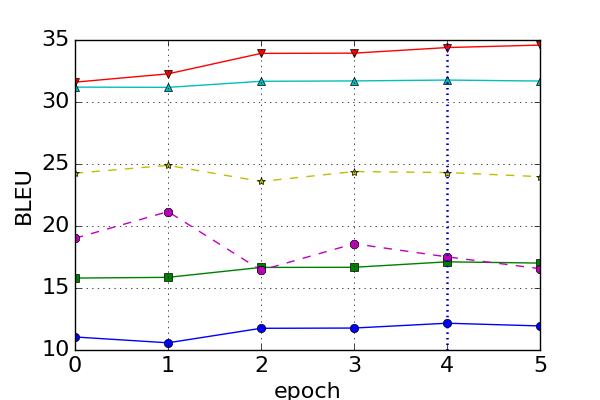
\includegraphics[width=\textwidth]{./img/adam/pp_abs_dev}
        \caption{pubPsych abstracts (dev)}
        \label{fig:pp_abs_dev}}
    \end{subfigure}
    \begin{subfigure}[b]{0.45\textwidth}
        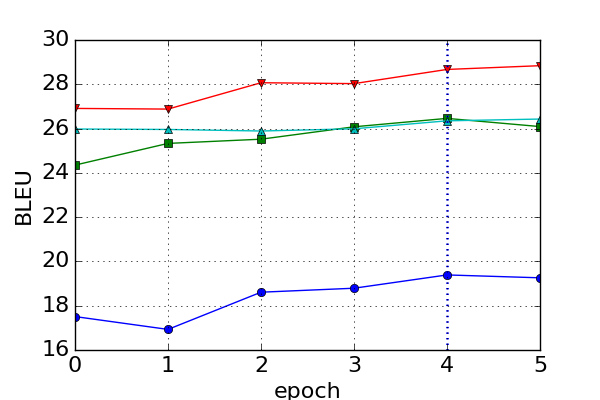
\includegraphics[width=\textwidth]{./img/adam/pp_abs_test}
        \caption{pubPsych abstracts (test)}
        \label{fig:pp_abs_set}
    \end{subfigure}
    \begin{subfigure}[b]{0.45\textwidth}
        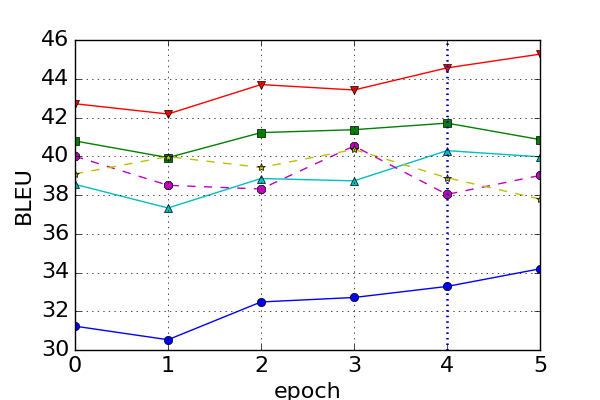
\includegraphics[width=\textwidth]{./img/adam/pp_title_test}
        \caption{pubPsych titles (test)}
        \label{fig:pp_tit}
    \end{subfigure}
    \begin{subfigure}[b]{0.45\textwidth}
        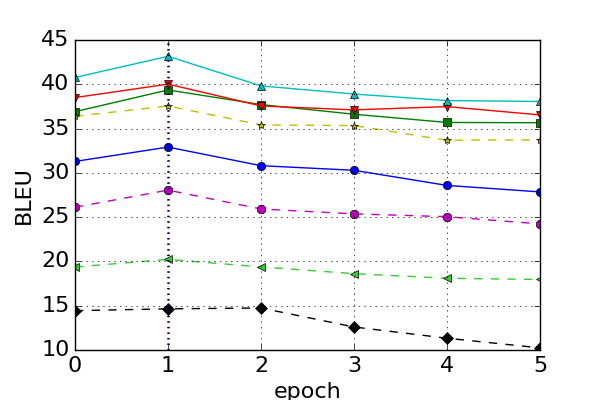
\includegraphics[width=\textwidth]{./img/adam/emea_dev}
        \caption{EMEA (dev)}
        \label{fig:emea_dev}
    \end{subfigure}
    \begin{subfigure}[b]{0.45\textwidth}
        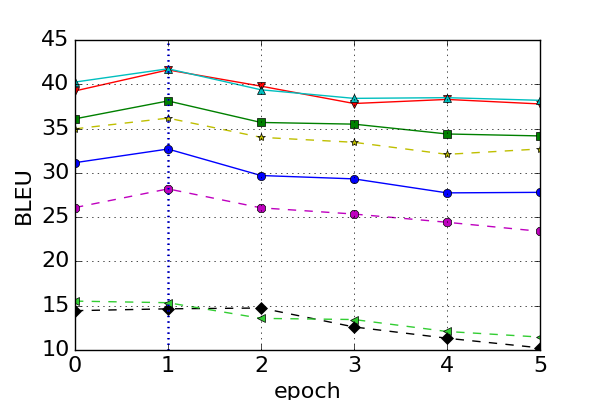
\includegraphics[width=\textwidth]{./img/adam/emea_test}
        \caption{EMEA (test)}
        \label{fig:emea_test}
    \end{subfigure}
    \begin{subfigure}[b]{0.45\textwidth}
        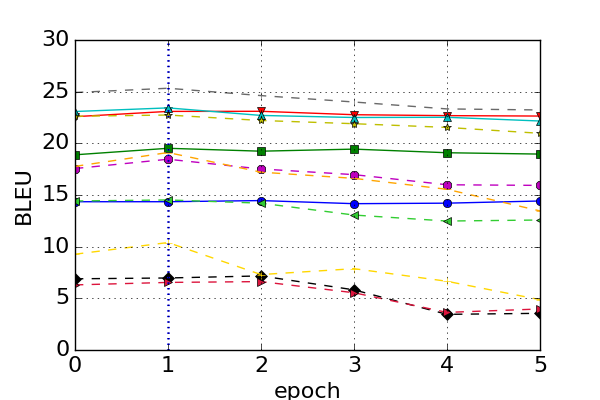
\includegraphics[width=\textwidth]{./img/adam/newstest}
        \caption{news-test}
        \label{fig:news-test}
    \end{subfigure}
    \begin{subfigure}[b]{.9\textwidth}
		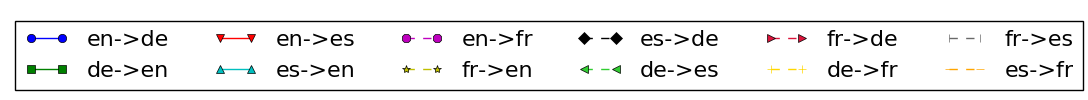
\includegraphics[width=\textwidth]{./img/adam/leg}    
    \end{subfigure}
    \caption{Evolution of domain adaptation through five epochs using the pubPsych adaptation corpus. Dashed lines indicate missing language pairs from adaptation data.}\label{fig:adapt_epochs}
\end{figure}

Figure~\ref{fig:adapt_epochs} displays the evolution of the NMT system throughout the 5 adaptation epochs. The figure is broken down by dataset, and different lines correspond to source-language pair combinations. Regarding the change in translation quality, several observations can be made. First, there are two different trends to be observed that depend on the type of the test data. It can be said in general that on in-domain datasets, the system's performance keeps improving until the fourth or fifth epoch. In most cases, the performance starts decreasing at the fourth epoch (a phenomenon that can be explained by overfitting). In the case of the three close- and out-of-domain datasets, however, the results saturate after one epoch of adaptation, and worsen after this point. The explanation for this behavior is that the overfitting takes effect much earlier due to the mismatch between the domain of the adaptation and test sets. Furthermore, this trend is repeated in the case of in-domain test sets for the language pair that is underrepresented in the adaptation set ($en$--$fr$, only titles are available). This is caused by the fact that even though the new data is beneficial, in this case its quality is inferior to the original training data, as that set contains sufficient parallel data for this language pair. Because of this, while one epoch of adaptation has positive effects, further training leads to decreasing quality.

% From this experiment we can draw several preliminary conclusions to determine the direction of further steps and more detailed analysis. Firstly, it is clear that the transfer learning approach to domain adaptation is a viable one in the case of this particular system and available adaptation dataset. Secondly, it helps us determine the number of adaptation epochs where the performance of the adapted systems is expected to be the best. On in-domain data, for the majority of language pairs this lies at four additional epochs. 
In the light of the previous analysis, we choose to test our systems using the model after fourth epoch in the adaptation process. Domain adaptation can even be beneficial for translating data that is not strictly in-domain or out-of-domain. In this case, however, we use systems that have only been adapted for one additional epoch of training. Similarly, this seems to be the best point in training for translating in-domain texts between language pairs that do not have any or sufficient parallel data in the adaptation set.

% 
% Regarding the achievable performance improvement, the results are displayed in Table~\ref{tab:indoma} to \ref{tab:indomb}, in the blocks marked as NMT PP. Arrows represent significant changes with respect to the baseline performance (NMT BL) as calculated by the bootstrap resampling method~\cite{koehn2004statistical} implemented in Moses\footnote{\url{https://github.com/moses-smt/mosesdecoder/blob/master/scripts/analysis/bootstrap-hypothesis-difference-significance.pl}}. Statistical significance is indicated at $p=0.005$. The evaluations are performed after 1 and 4 epochs of adaptation respectively, depending on the test set as described above. On the in-domain data we obtain significant improvement in all cases, that generally lies between 1 and 2 BLEU scores. In certain cases the improvements are not significant, most notably on the $en$--$fr$ language pair where there is no adaptation data available (other cases are $es\rightarrow en$ on the \textit{pubPsych abstracts} sets, and $de\rightarrow en$ on \textit{pubPsych titles}). On the \textit{pubPsych titles} test set, the performance is significantly worse in the case of the $en\rightarrow fr$ direction. The average relative improvements (Avg.) and their standard deviations (SD) are displayed in Table~\ref{tab:reli-indom}, broken down by test set.



\newcommand{\da}{$\downarrow$}
\newcommand{\ua}{$\uparrow$}

\begin{table}
% 	\flushleft{\bf $en\rightarrow de$\\ \smallskip}
	\flushleft{\hspace*{2.4cm} \bf $en2de$  \hspace*{5.6cm} $de2en$  \\ \smallskip}	
	\small
	\begin{tabular}{lrrrrr rrrrr}
		\toprule
		&  \mc{1}{c}{\bf Abstracts} & \mc{1}{c}{\bf Titles} & \mc{1}{c}{\bf EMEA} & \mc{1}{c}{\bf News} 
		&  \mc{1}{c}{\bf Abstracts} & \mc{1}{c}{\bf Titles} & \mc{1}{c}{\bf EMEA} & \mc{1}{c}{\bf News}\\
% 		\toprule
% 		& \mc{1}{c}{\textit{PP abs. (dev)}} & \mc{1}{c}{\bf Abstracts} & \mc{1}{c}{\bf Titles} & \mc{1}{c}{\textit{EMEA (dev)}} & \mc{1}{c}{\bf EMEA} & \mc{1}{c}{\bf News}\\
		\midrule
		NMT & 11.05 & 31.23 &    31.15 & 14.35                              &               15.80 & 40.79 & 36.10 & 18.89 \\
		NMTpp & \ua \textbf{12.16} & \ua 33.28 &  32.69 & 14.35               &  \ua \textbf{17.11} & 41.70 & \ua \textbf{38.12} & 19.52\\
		\midrule                                                               
		NMTwp5   & \da 10.04 & 30.44    &  \da 26.70 & \da 13.17                  &  \da 15.01 & 40.59 &  \da 34.28 & 19.26\\
		NMTwp10  & \da 9.80 & \da 28.59 &  \da 26.67 & \da 13.25                  &  15.12 & \da 39.24 &  \da 33.66 & \ua 19.37\\
		NMTwp30  & \da 7.76 & \da 23.12 &  \da 25.95 & \da 13.12                  &  15.34 & \da 37.86 &  \da 33.18 & 18.39\\
		\midrule
		NMTmrg5  &\ua 11.74\da & \ua 33.60          & \da 28.32\da &  14.34     &  \ua 16.49\da &  41.34 &  \da 34.84\da &  19.26\\
		NMTmrg10 &\ua 11.69\da & \ua 33.89          & \da 29.54\da &  14.62     &  \ua 16.66\da & \ua \textbf{42.02} &  \da 34.81 & \ua \textbf{19.46}\\
		NMTmrg30 &   \ua 11.96 & \ua \textbf{33.97} & \da 27.33\da &  13.46\da  &  \ua 16.95 &  41.44  & \da 33.03\da &  19.41\\
		\bottomrule
	\end{tabular}
	
% 	\flushleft{\bf $de\rightarrow en$\\ \smallskip}
% 	\begin{tabular}{lrrrrrr}
% 		\toprule
% 		& \mc{1}{c}{\textit{PP abs. (dev)}} & \mc{1}{c}{\bf Abstracts} & \mc{1}{c}{\bf Titles} & \mc{1}{c}{\textit{EMEA (dev)}} & \mc{1}{c}{\bf EMEA} & \mc{1}{c}{\bf News}\\
% 		\midrule
% 		NMT &               15.80 & 40.79 & & 36.10 & 18.89 \\
% 		NMTpp &  \ua \textbf{17.11} & 41.70 & & \ua \textbf{38.12} & 19.52\\
% 		\midrule
% 		NMTwp5  &    \da 15.01 & 40.59 &  \da 34.28 & 19.26\\
% 		NMTwp10 &    15.12 & \da 39.24 &  \da 33.66 & \ua 19.37\\
% 		NMTwp30 &    15.34 & \da 37.86 &  \da 33.18 & 18.39\\
% 		\midrule
% 		NMTmrg5  & \ua 16.49\da &  41.34 &  \da 34.84\da &  19.26\\
% 		NMTmrg10 & \ua 16.66\da & \ua \textbf{42.02} &  \da 34.81 & \ua \textbf{19.46}\\
% 		NMTmrg30 & \ua 16.95 &  41.44  & \da 33.03\da &  19.41\\
% 		\bottomrule
% 	\end{tabular} 
	\caption{BLEU scores for the different systems used to domain-adapt the general NMT system for the phsycological domain German--English. Arrows mark statistical significance (see text) and best results on each test set are shown in bold (in case of significant improvements).}
	\label{tab:nmtEnDe}               
\end{table}


Here, the arrows after the BLEU scores indicate significant differences ($p=0.005$) when compared to the adapted results achieved in the PP adaptation scenario, while the ones before the numbers stand for significant differences with respect to the baseline system.

Tables \ref{tab:nmtEnDe}--\ref{tab:xfr} show the BLEU scores for the different systems and language pairs. Arrows before BLEU scores represent significant changes with respect to the baseline performance (NMT) as calculated by the bootstrap resampling method implemented in Moses~\cite{koehn04}. Statistical significance is indicated at $p=0.005$. Arrows after the BLEU scores indicate significant differences when compared to the adapted results achieved by NMTpp. The evaluations are performed after 1 and 4 epochs of adaptation respectively, depending on the test set as described above. With the NMTpp system on the in-domain data, we obtain significant improvement in all cases, that generally lies between 1 and 2 BLEU scores. In certain cases the improvements are not significant though, most notably on the $en$--$fr$ language pair where there is no adaptation data available (other cases are $es\rightarrow en$ on the \textit{pubPsych abstracts} sets, and $de\rightarrow en$ on \textit{pubPsych titles}). 

\begin{table}
% 	\centering
	\flushleft{\hspace*{2.4cm} \bf $en2es$  \hspace*{5.8cm} $es2en$  \\ \smallskip}	
	\small
	\begin{tabular}{lrrrrr rrrrr}
		\toprule
		&  \mc{1}{c}{\bf Abstracts} & \mc{1}{c}{\bf Titles} & \mc{1}{c}{\bf EMEA} & \mc{1}{c}{\bf News} 
		&  \mc{1}{c}{\bf Abstracts} & \mc{1}{c}{\bf Titles} & \mc{1}{c}{\bf EMEA} & \mc{1}{c}{\bf News}\\
		\midrule
		NMT &  31.60    & 42.71 & 39.25 & 22.58                                         & 31.20 & 38.55  & 40.25 & 23.08\\
		NMTpp & \ua 34.39 & \ua 44.56 & \ua \textbf{41.62} & \ua 23.09                    & 31.77     & \ua 40.29    & 41.75 & 23.43\\
		\midrule
		NMTwp5  &  31.25 & 41.05 &  \da 36.49 & \da 21.74                                     & \da 30.12 &     38.16 & \da 36.91 & \ua 23.85\\
		NMTwp10 &  32.09 & 40.91 &  \da 36.17 & \da 21.92                                     & \da 30.35 &     37.20 & \da 37.56 & \ua 23.73\\
		NMTwp30 &  31.73 & \da 40.26 & \da 36.11 & 22.49                                      & \da 30.10 & \da 35.47 & \da 36.45 & \ua \textbf{23.94}\\
		\midrule
		NMTmrg5  & \ua 34.02 & \ua\textbf{45.31}  & \da 36.79\da & \ua 23.49                & 32.22 & \ua 40.25 &  \da 38.05\da & 23.49\ua \\
		NMTmrg10 & \ua 33.44 & \ua 44.72 & \da 38.58\da & \ua \textbf{23.68}\ua             & 32.21 & \ua \textbf{40.37}  & \da 38.67\da &  23.36\da \\
		NMTmrg30 & \ua \textbf{34.60} & \ua 44.98 & \da 36.42\da & \ua 23.43                & 31.91 & 40.19 & \da 37.52\da & \ua 23.78\ua \\
		\bottomrule
	\end{tabular}
	
% 	\flushleft{\bf $es\rightarrow en$\\ \smallskip}
% 	\begin{tabular}{lrrrrr}
% 		\toprule
% 		& \mc{1}{c}{\bf Abstracts} & \mc{1}{c}{\bf Titles} &  \mc{1}{c}{\bf EMEA} & \mc{1}{c}{\bf News}\\
% 		\midrule
% 		NMT    & 31.20 & 38.55  & 40.25 & 23.08\\
% 		NMTpp    & 31.77     & \ua 40.29    & 41.75 & 23.43\\
% 		\midrule
% 		NMTwp5       & \da 30.12 &     38.16 & \da 36.91 & \ua 23.85\\
% 		NMTwp10      & \da 30.35 &     37.20 & \da 37.56 & \ua 23.73\\
% 		NMTwp30      & \da 30.10 & \da 35.47 & \da 36.45 & \ua \textbf{23.94}\\
% 		\midrule
% 		NMTmrg5    & 32.22 & \ua 40.25 &  \da 38.05\da & 23.49\ua \\
% 		NMTmrg10   & 32.21 & \ua \textbf{40.37}  & \da 38.67\da &  23.36\da \\
% 		NMTmrg30   & 31.91 & 40.19 & \da 37.52\da & \ua 23.78\ua \\
% 		\bottomrule
% 1	\end{tabular}
	\caption{As Table \ref{tab:nmtEnDe} for the Spanish--English language pair.}
	\label{tab:nmtEnEs}               
\end{table}

\begin{table}
% 	\centering
	\flushleft{\hspace*{2.4cm} \bf $en2fr$  \hspace*{5.6cm} $fr2en$  \\ \smallskip}	
	\small
	\begin{tabular}{l rrrr rrrr}
		\toprule
		& \mc{1}{c}{\bf Abstracts} & \mc{1}{c}{\bf Titles} &  \mc{1}{c}{\bf EMEA} & \mc{1}{c}{\bf News}
		& \mc{1}{c}{\bf Abstracts} & \mc{1}{c}{\bf Titles} &  \mc{1}{c}{\bf EMEA} & \mc{1}{c}{\bf News}\\
		\midrule
		NMT & 19.01 & 40.00    &  26.08 & 17.56                            & 24.60 & 39.09 &  34.97 & 22.62\\
		NMTpp & \ua 21.16 & \da 38.35 &  \ua \textbf{28.19} & 18.46          & 24.89 & 39.98 &  36.18 & \ua 22.74\\
		\midrule
		NMTwp5  & \ua 20.96 & \da 36.41 &  25.33 & \ua 18.94                     & 23.39 & \ua \textbf{40.84} & 33.67 & \ua 23.12\\
		NMTwp10 & \ua 22.41 & \da 35.39 &  25.36 & \ua 19.20                     & 22.41 & 39.22 & \da 32.85 & 22.85\\
		NMTwp30 & \ua \textbf{22.87} & \da 35.03 & 25.83 & \ua \textbf{19.28}    & 23.51 & 38.44 & 32.03 & \ua \textbf{23.38}\\
		\midrule
		NMTmrg5  &     19.41\da &  39.36 &  25.15\da    & \ua 18.38\da         & 24.60 &  39.33    & \da 32.91\da & 22.78\ua\\
		NMTmrg10 &     18.71\da &  38.87 & \ua 26.22\da & \ua 18.89\ua         & 24.92 &  38.16\da &  33.05 &  22.51\\
		NMTmrg30 & \ua 21.40\ua &  38.89 & \da 25.60\da & \ua 18.94\ua         & 24.25 &  40.99    & \da 32.87 &  22.19\da\\
		\bottomrule 
	\end{tabular}
	
% 	\flushleft{\bf $fr\rightarrow en$\\ \smallskip}
% 	\begin{tabular}{lrrrrr}
% 		\toprule
% 		& \mc{1}{c}{\bf Abstracts} & \mc{1}{c}{\bf Titles} & \mc{1}{c}{\textit{EMEA (dev)}} & \mc{1}{c}{\bf EMEA} & \mc{1}{c}{\bf News}\\
% 		\midrule
% 		NMT   & 24.60 & 39.09 &  34.97 & 22.62\\
% 		NMTpp   & 24.89 & 39.98 &  36.18 & \ua 22.74\\
% 		\midrule
% 		NMTwp5      & 23.39 & \ua \textbf{40.84} & 33.67 & \ua 23.12\\
% 		NMTwp10     & 22.41 & 39.22 & \da 32.85 & 22.85\\
% 		NMTwp30     & 23.51 & 38.44 & 32.03 & \ua \textbf{23.38}\\
% 		\midrule
% 		NMTmrg5   & 24.60 &  39.33    & \da 32.91\da & 22.78\ua\\
% 		NMTmrg10  & 24.92 &  38.16\da &  33.05 &  22.51\\
% 		NMTmrg30  & 24.25 &  40.99    & \da 32.87 &  22.19\da\\
% 		\bottomrule
% 	\end{tabular}
	
	\caption{As Table \ref{tab:nmtEnDe} for the French--English language pair. Notice that we have not used direct parallel data for this language pair during the transfer learning phase.}
	\label{tab:nmtEnFr}               
\end{table}


\begin{table}
 	\centering
	\flushleft{\hspace*{2.4cm} \bf $es2de$  \hspace*{2.2cm} $de2es$  \\ \smallskip}	
	\small
% 	\flushleft{\bf $es\rightarrow de$\\ \smallskip}
	\begin{tabular}{lrr rr}
		\toprule
		&  \mc{1}{c}{\bf EMEA} & \mc{1}{c}{\bf News} &  \mc{1}{c}{\bf EMEA} & \mc{1}{c}{\bf News} \\
		\midrule
		NMT   & 15.52 & 6.89                       & 20.57 & 14.42\\
		\midrule
		NMTpp   & \da 15.34 & 6.97                   & 20.90 & 14.52\\
		\midrule
		NMTwp5      &  16.58 & \ua 9.78                  &\da 20.55 & \ua \textbf{15.03}\\
		NMTwp10     &  16.84 & \ua 9.73                  &\ua 20.65 & 14.62\\
		NMTwp30     &  16.39 & \ua 9.94                  &\da 19.45 & \da 13.98\\
		\midrule
		NMTmrg5  & \textbf{ 17.46}\ua & \ua 10.71\ua   & \da 20.43\da &  14.75\ua \\
		NMTmrg10 & 17.71 & \ua 10.68\ua                & \da 20.05    &  14.90\ua\\
		NMTmrg30 & 17.12 & \ua \textbf{10.76}\ua       & \da 20.21\da & 14.96\ua\\
		\bottomrule		
	\end{tabular}
% 	\flushleft{\bf $de\rightarrow es$\\ \smallskip}
% 	\begin{tabular}{lrrr}
% 		\toprule
% 		 & \mc{1}{c}{\bf EMEA} & \mc{1}{c}{\bf News}\\
% 		\midrule
% 		NMT   & 20.57 & 14.42\\
% 		\midrule
% 		NMTpp   & 20.90 & 14.52\\
% 		\midrule
% 		NMTwp5      &\da 20.55 & \ua \textbf{15.03}\\
% 		NMTwp10     &\ua 20.65 & 14.62\\
% 		NMTwp30     &\da 19.45 & \da 13.98\\
% 		\midrule
% 		NMTmrg5   & \da 20.43\da &  14.75\ua \\
% 		NMTmrg10  & \da 20.05    &  14.90\ua\\
% 		NMTmrg30  & \da 20.21\da & 14.96\ua\\
% 		\bottomrule
% 	\end{tabular}
	\caption{As Table \ref{tab:nmtEnDe} for Spanish--German. Notice that we have not used direct parallel data for this language pair when training the NMT system or during the transfer learning phase.}
	\label{tab:nmtEsDe}               
\end{table}


\begin{table}
	\begin{center}
	\flushleft{\hspace*{2.7cm} \bf $es2fr$~~~~~$fr2es$~~~~~$de2fr$~~~~$fr2de$\\ \smallskip}
	\small
	\begin{tabular}{lr|r|r|r}
		\toprule
% 		& \mc{1}{c}{\bf News} & \mc{1}{c}{\bf News} & \mc{1}{c}{\bf News} & \mc{1}{c}{\bf News} \\
		NMT & 17.77 & 24.92 & 9.27 & 6.30\\
		\midrule
		NMTpp & \ua 19.11 & 25.33 & \ua 10.40 & 6.54\\
		\midrule
		NMTwp5 & \ua \textbf{21.30} & \ua 25.77  & \ua 11.29 & \ua 10.14\\
		NMTwp10 & \ua \textbf{21.30} & \ua 25.92 & \ua \textbf{10.98} & \ua 10.01\\
		NMTwp30 & \ua 21.28 & \ua 26.15 & 8.23 & \ua 9.01\\
		\midrule
		NMTmrg5 & \ua 20.21\ua & \ua 25.48\ua & \ua 10.53\ua & \ua \textbf{10.41}\ua\\
		NMTmrg10 & \ua 20.88\ua & \ua 25.82\ua & \ua 10.97\ua & \ua 10.03\ua\\
		NMTmrg30 & \ua 20.80\ua & \ua \textbf{26.18}\ua & 9.78\da & \ua 9.44\ua\\
		\bottomrule
	\end{tabular}
	 
	\end{center}
	\caption{BLEU scores for the different systems used to domain-adapt the general NMT system for the phsycological domain  in the $es$--$fr$ and $de$--$fr$ language pairs. Notice that at this point of the project we only have available the out-of-domain news test set.}	
	\label{tab:xfr}
\end{table}

When enriching our data with parallel sentences extracted from Wikipedia in the health domain, we see that for most translation directions and test sets the results are 1--2 BLEU points worse compared to the baseline system's performance, often reaching significant levels. Certain scenarios perform slightly better than the unadapted system, the improvement, however, is usually not significant compared to the baseline. The quality of the data seems to be not high enough to significantly improve the in-domain performance. It has to be noted that in addition to the lower quality, the actual domain coverage of the data does not necessarily align completely with that of the test sets. This is backed up by the fact that adapting with the WP data leads to significant improvements on the out-of-domain \textit{news-test2013} dataset (except for $en\rightarrow es$ and $en\rightarrow de$), while on the close-domain EMEA test sets we observe a behavior similar to the strictly in-domain \textit{pubPsych} sets. As we aimed for covering a large number of articles when extracting from the health and psychology domains, the automatic adaptation set contains many parallel sentences that are only slightly related to these topics and they have proben not to be useful.

Since in this setting we have available data for language pairs that are under- or zero-resourced in either the PP data set, or even the general NMT system, the \textit{Wikipedia} extractions have a clear positive effect for these language pairs and the adapted systems often overperform the ones that have been adapted on \textit{pubPsych} data. The conclusions obtained with the NMTwp systems are also valid for NMTmrg systems.

% The general trend in case of worsening performances is proportionate to the adaptation datasets' size: as it increases, the results get worse, reaching significant levels of difference for the WP30 in the case of $en\rightarrow es$ and $de\rightarrow en$ on certain test sets (for $de\rightarrow en$ it already happens at WP10 for the \textit{pubPsych titles} test set).  The noteworthy exception is the $en\rightarrow fr$ direction on the \textit{pubPsych titles} test set, where the top-5,000 set already drastically worsens the translation quality (more than 3.5 points of drop), and one can observe a decreasing trend in terms of BLEU score as the size of the dataset increases. Conversely, the reverse direction $fr\rightarrow en$ showcases significant improvement on the same test set for WP5. 

% There is one case, however, when the adaptation with the automatic extractions yields results that are significant improvements with regard to the baseline performance. Interestingly enough, this also happens with the $en\rightarrow fr$ direction, on the abstract test set. In this case, we can observe a steady improvement as the size of the dataset increases. All results overperform the adaptation results with the PP adaptation set at the same number of epochs (that has no data for abstracts for this language pair). On the other hand, the reverse direction $fr\rightarrow en$ does not demonstrate the same behavior on the same test set, as results get worse using this adaptation data, and in this case adaptation with the parallel PP data yields a somewhat better performance (even though it is still worse than the baseline's). These differences, however, are not significant in any of these cases.



\section{Additional Experiments}
\label{s:moreExperiments}



\section{Conclusions}
\label{s:conclusions}

Regarding this set of experiments, we can draw several conclusions. Firstly, as in most cases we cannot achieve significant improvement on the in-domain test sets, it can be concluded that using automatically extracted adaptation sets from \textit{Wikipedia} without any additional clean data is generally not useful for NMT systems, as its quality is not high enough to significantly improve the in-domain performance. It has to noted that in addition to the lower quality, the actual domain coverage of the data does not necessarily align completely with that of the test sets. This is backed up by the fact that adapting with the WP data leads to significant improvements on the out-of-domain \textit{news-test2013} dataset (except for $en\rightarrow es$ and $en\rightarrow de$), while on the close-domain EMEA test sets we observe a behavior similar to the strictly in-domain \textit{pubPsych} sets. As we aimed for covering a large number of articles when extracting from the health and psychology domains, the automatic adaptation set contains many parallel sentences that are only slightly related to these topics. Narrowing the search criteria could be a future possibility, however, this could lead to losing a great number of high-quality parallel sentences, and therefore would not necessarily lead to an improvement.

%
% ---- Bibliography ----
%
\addcontentsline{toc}{section}{References}
\bibliographystyle{plain}
\bibliography{genericMT}


\end{document}
